\subsection{IllustrisTNG}
%Add footnote with IllustrisTNG webpage
IllustrisTNG \footnote{https://www.tng-project.org/} is the follow-up project after the success of the Illustris simulations. It is a huge project, built upon a magneto-hydrodynamical cosmological simulation code with added physical processes on a subgrid level \parencite{Weinberger2016}. Adding physical processes like gas radiation, star formation, stellar feedback through supernova explosions, supermassive blackhole accretion and magnetic fields are essential to model galaxy formation and evolution, and allows a much better comparison to reality. The data output from the simulations is extensive, and is not meant to be analysed all in one go, but rather through a series of analyses, each targeting a specific scientific question. 


\subsubsection{The simulations}
The IllustrisTNG project includes 18 different simulations with varying resolutions, spatial size and included physics. There are three main simulations that differ in volume and resolution, and the details of these are summed up in Table \ref{TNG}. Each of the main simulations have been run at three different resolution levels, which makes it possible to study how changing only the resolution in a given simulation affects the outcome. TNG100 has a physical box volume of $110.7^3 \, $Mpc$^3$, and a baryonic particle resolution of $1.4 \times 10^6 M_{\odot}$, while the TNG300 simulation has a volume of $302.6^3 \, $Mpc$^3$ and a baryonic particle resolution of $1.1 \times 10^7 M_{\odot}$. The TNG50 data is actually not yet available, but it is expected soon, and provides a much higher resolution in a smaller box size. In this project, a large statistical sample of galaxies was needed, as well as detailed structure of the inner part of the galaxies to calculate the different properties, so the TNG100 simulation was the ideal middle ground with respect to size and resolution. The TNG100-1 simulation data has been used throughout the project, which is the highest available resolution for TNG100. A visual representation of parts of the simulations can be seen in Figure \ref{tng_illustration}.

\begin{figure}
    \centering
    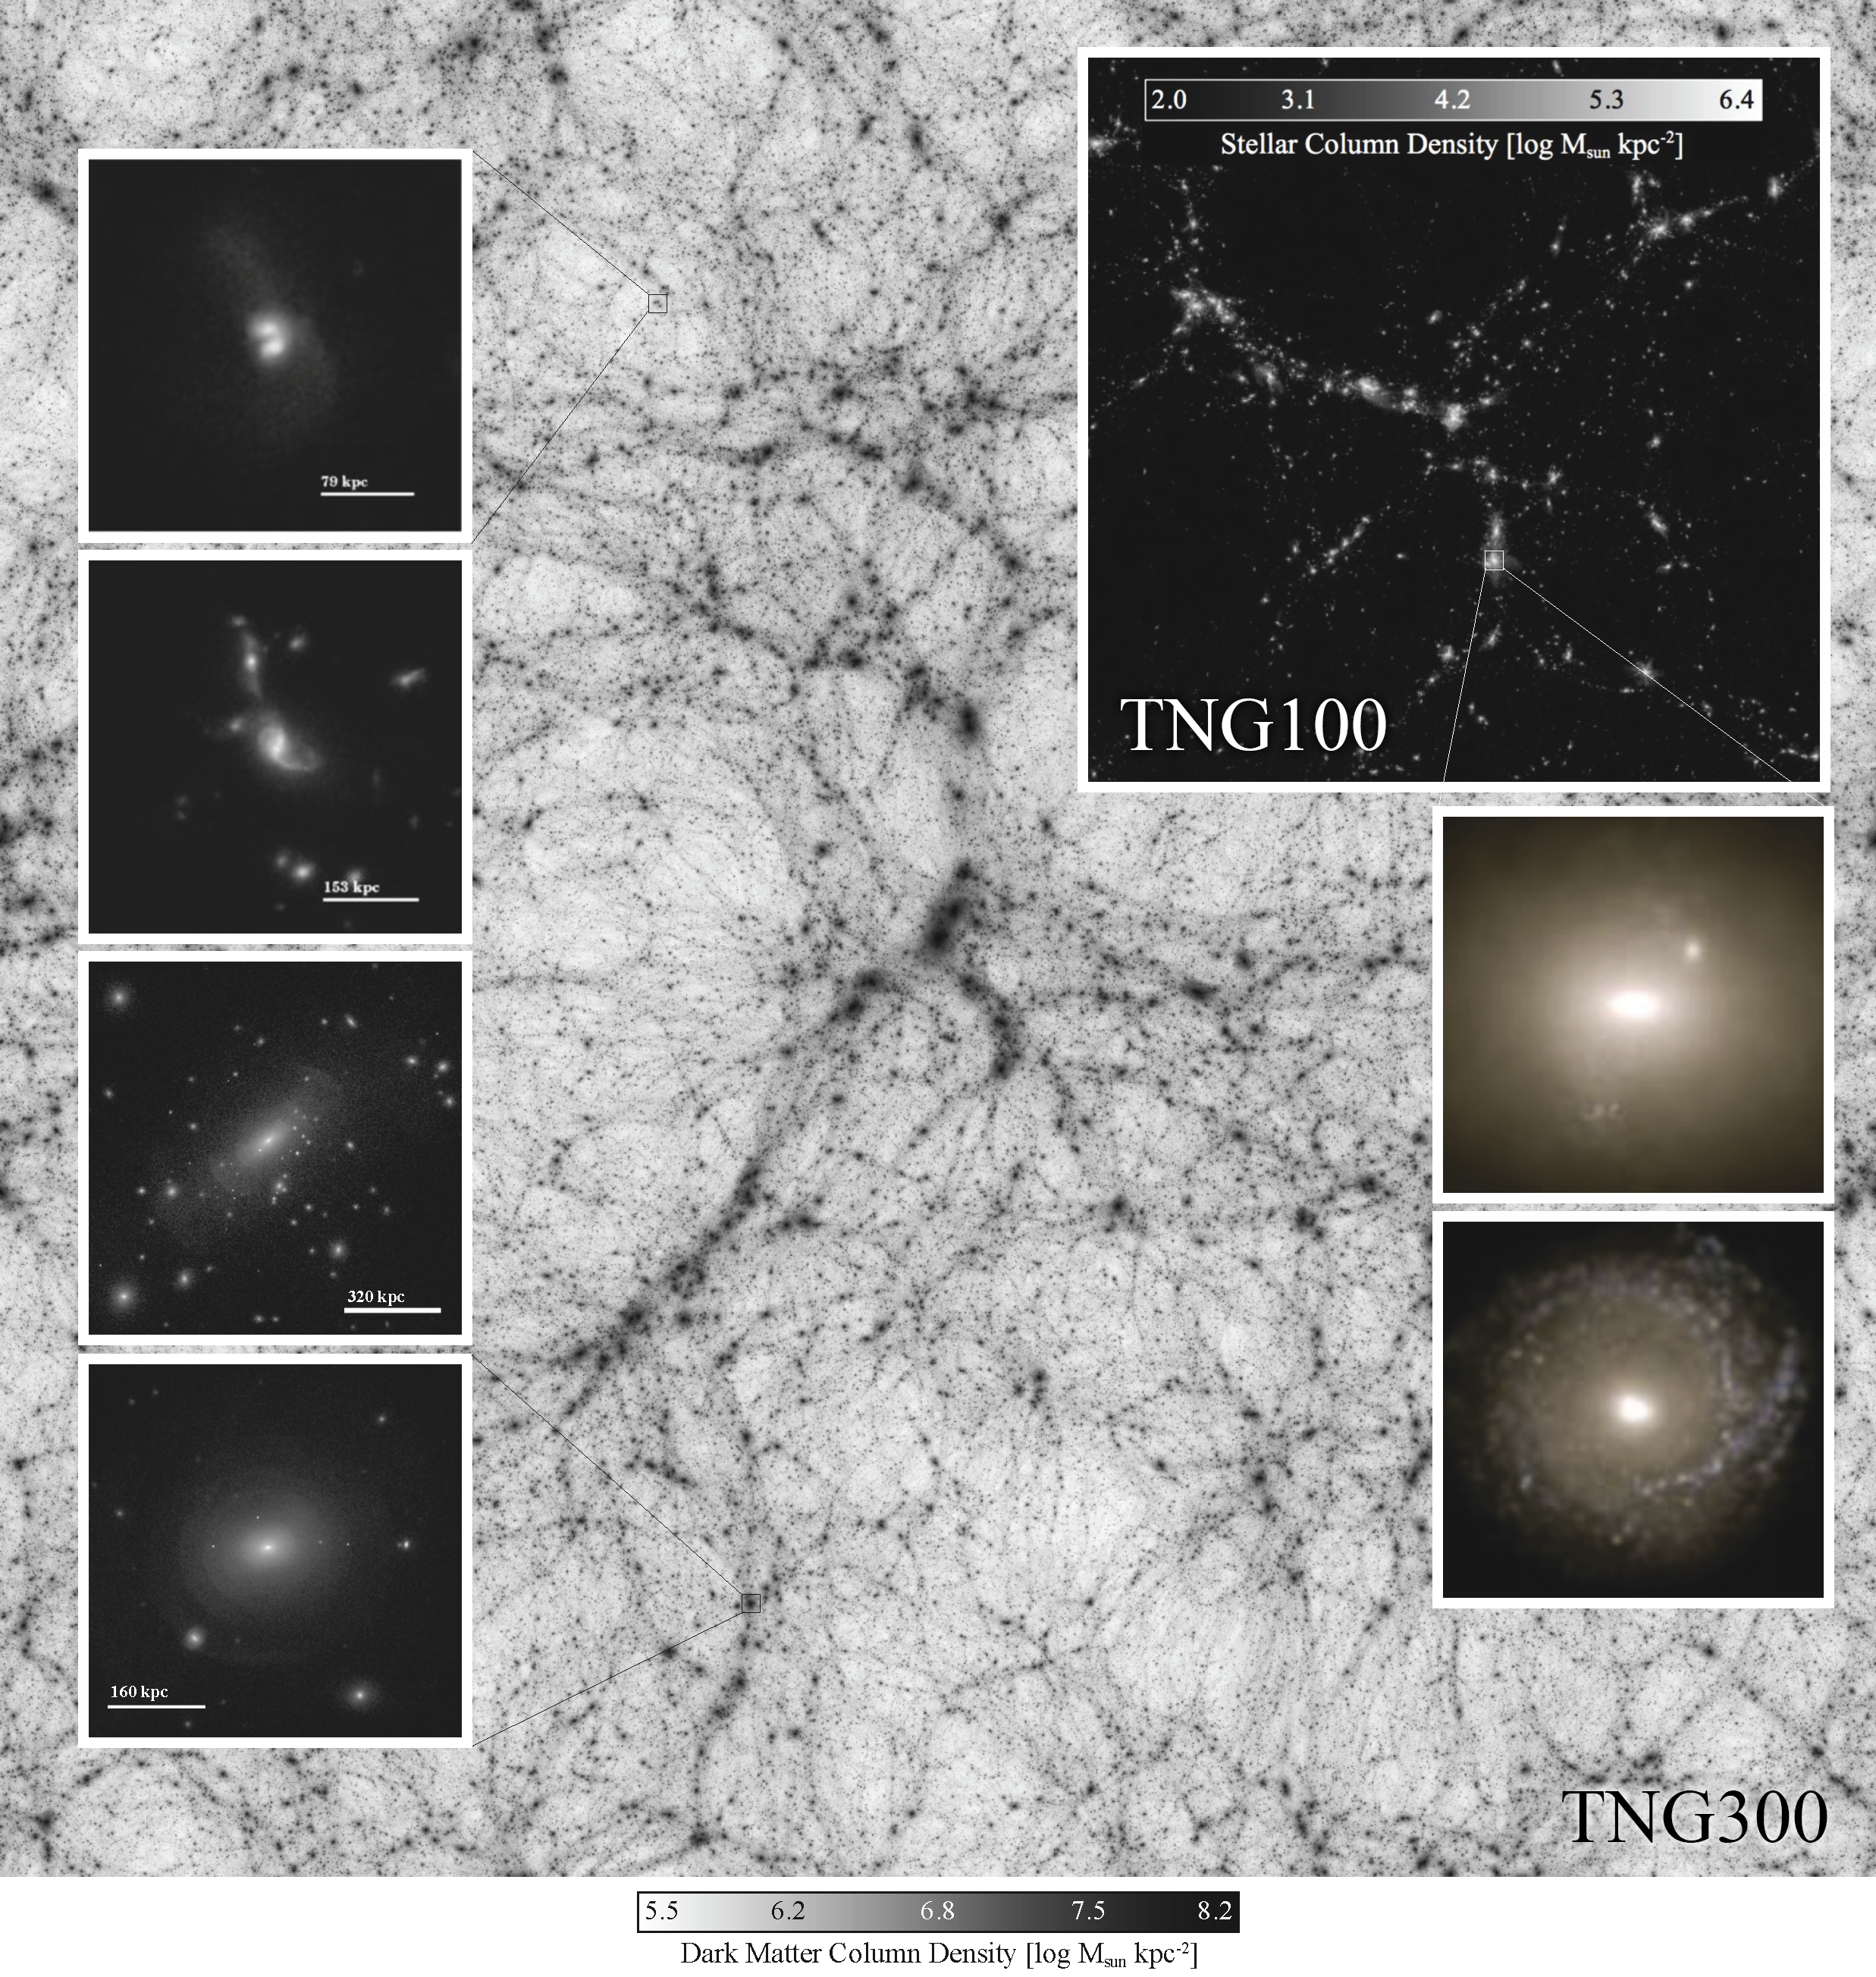
\includegraphics[width=0.9\textwidth]{images/TNG.png}
    \caption{A composite image that illustrates the two simulations TNG100 and TNG300. In the background is the dark matter distribution for the whole TNG300 volume. In the upper right is the stellar mass distribution across the entire TNG100 volume. The panels on the left show galaxy-galaxy interactions, while the panels on the right show the stellar light projections of two $z=0$ galaxies. Credit: TNG Collaboration}.
    \label{tng_illustration}
\end{figure}

\begin{table}
\begin{center}
\begin{tabular}{ l| c c c c c } 
 \hline
 \hline
   &  Volume [$Mpc^3$] & $N_{DM}$ & $m_{DM}$ [$M_{\odot}$] & $m_{baryon}$ [$M_{\odot}$] \\
 \hline
 TNG50 & $51.7^3$ & $2163^3$ & $4.5 \times 10^5 $ & $8.5 \times 10^4 $ \\ 
 TNG100 & $110.7^3$ & $1820^3$ & $7.5 \times 10^6 $ & $1.4 \times 10^6 $  \\ 
 TNG300 & $302.6^3$ & $2500^3$ & $5.9 \times 10^7 $ & $1.1 \times 10^7 $  \\ 
 \hline 
 \end{tabular}
\end{center}
\caption{The simulation details for the three main TNG simulations. $N_{DM}$ is the amount of dark matter particles. $m_{DM}$ and $m_{baryon}$ is the mass of the dark matter and baryonic particles, respectively.}
 \label{TNG}
\end{table}

\subsubsection{Data cataloges}
All the Illustris-TNG data is publically available online at the TNG webpage. The data products that are available for each simulation are snapshots, group catalogs and merger trees as well as some supplementary data sets. There are 100 snapshots for each run, which are taken at specific redshifts. They include all the particles in the whole volume of the simulation, with 20 of them including all the particle fields for each particle as well. There are five different particle types, and each particle has its properties stored as particle fields. These fields include information like position, kinematic data and atomic/chemical composition. 


The group catalogs provide a convenient way to quickly access already calculated properties of the different halos and subhalos instead of dealing with all the particles in a snapshot. This saves a lot of time and effort, but gives the user less control over what can be analysed. In future work, it might be interesting to do the calculations directly from the snapshots myself. There is one group catalog for each snapshot, and this includes two types of objects, Friends-of-Friends (FoF) and Subfind. The FoF catalog contains all the halos, and the Subfind catalog contains all the subhalos for each halo. Each subhalo has a parent halo, and the largest subhalo in each halo is the central subhalo. The merger trees data products contain the merger history of each subhalo.

This project makes use of the group catalogs for the $z = 0$ snapshot in TNG100-1, as we want to compare the output data to observations of the local (present time) universe.

\subsubsection{Selection criteria} %badtitle

The TNG documentation recommends filtering out all subhalos that are flagged with the $SubhaloFlag$ field, and so these were cut from the data. These are most probably subhalos of non-cosmological origin, and so should not be considered real galaxies.

For most of the relations covered in this project, it is desirable to only use the central galaxies in each halo. This is because satellite galaxies are more affected by their environment, which in turn affects the kinematic and structural properties of the galaxy. This will naturally lead to a scatter in the galaxy scaling relations that are being studied, which central galaxies will not display. The FoF catalog contains the index for the largest subhalo in each halo, so combining this information with the Subfind catalog allows one to create a subset of the data that contains only the central galaxies.

Only galaxies with stellar mass greater than $10^9 M_{\odot}$ are used, except for the SHMR analysis, where galaxies with stellar mass down to $10^8 M_{\odot}$ are included. This is because smaller galaxies will have fewer stellar particles, and thus their structure is not necessarily reliably resolved.

\subsection{Observational data}
//Some general itroduction to observational data goes here

It is desirable to use the same observational data when comparing different scaling relations, however it has not been possible to do that. This is because we are analysing such different problems as stellar-to-halo mass and SMBH relations, which require very different kind of measurements. A compromise has been to use one main survey for the kinematic scaling relations. 

//fill in when you know more about this //

\subsubsection{SAMI Galaxy Survey}
The Sydney – Australian Astronomical Observatory Multi-Object Integral Field Spectrograph (SAMI) is mounted on the Anglo-Saxan telescope in Australia. The SAMI Galaxy Survey \footnote{https://sami-survey.org/} is a spectroscopic survey of a large sample of galaxies in the nearby universe ($z < 0.113$). The survey was started in 2013, and ended in 2018. There have been two major data releases, with the newest being Data Release Two (DR2) \parencite{Scott2018}. DR2 includes data for 1559 galaxies, which is about 50 \% of the full galaxy survey. The data products available are IFS data cubes and 2D maps, as well as catalogue data. Analysing data cubes and 2D maps falls outside the scope of this product, so catalogue data is used where possible. Some data is not available in the catalogues, but the direct results from research using the SAMI data has then been used.


\subsubsection{Other data sets}
//Write about the data sets for SHMR and SMBH
For the SHMR best fit models from two different abundance method papers were used in the comparison to TNG.

In \cite{Moster2012} a double power law was used to fit the data,

\begin{equation}
	M_{*}/M_{halo} = 2 N[(\frac{M}{M_1})^{-\beta}+(\frac{M}{M_1})^{\gamma}]^{-1},
\end{equation}
where N is a normalization parameter, $M_1$ is a characteristic mass and $\beta, \gamma$ are the slopes at the low and high-mass end respectively. The best fit for the four free parameters at redshift $z=0$ are given as $M_1 = 11.590 \pm 0.236$, $N = 0.0351 \pm 0.0058$, $\beta = 1.376 \pm 0.153$ and $\gamma = 0.608 \pm 0.059$.

\cite{Behroozi2013} improved the fit by using a power law for the high mass end, and a subpower law for the low mass end.

\begin{equation}
    \log(M_*(M_h)) = \log(\epsilon M_1) + f(\log(M_h/M_1)) -f(0),
\end{equation}
\begin{equation*}
    f(x) = -\log(10^{\alpha x}+1)+\delta \frac{(\log(1+\exp(x)))^\gamma}{1 +\exp(10^{-x})}
\end{equation*}

Here $M_1$ is a characteristic halo mass, $\delta$ is the strength of the subpower law, $\alpha$ is the power law slope for $M_h << M_1$ and $\gamma$ is the power law index for $M_h >> M_1$. The values for the parameters are $M_1 = 11.514\pm(0.053, 0.009)$, $\delta = 3.508 \pm (0.087, -0.369)$, $\alpha = -1.412 \pm (0.020, -0.105)$ and $\gamma = 0.316 \pm (0.076, -0.012)$.


//Moster, Behroozi, Tundo and Ferrarese

\subsection{Calculating properties}

\subsubsection{Cosmologies and property value representation} \label{cosmologies}
When making measurements of galaxy properties at cosmological distances, some assumptions about the underlying cosmology of the universe must be made. One of these assumptions is the value of the Hubble constant $H_0$, more commonly represented by $h$. This constant is also used when properties are calculated using a simulation. For IllustrisTNG, $H_0 = 100\,h\,$ km/s/Mpc with $ h = 0.6774$ and the explicit $h$-dependence of each property value is stated clearly in the documentation. For the SAMI data catalogue, no h-dependence is explicitly stated in the documentation or data release papers, but the Hubble constant used is given, $h = 0.7$.
\cite{Behroozi2013} uses $h = 0.7$ as well. In \cite{Moster2012} a value of $h = 0.704$ is chosen. For the BHMR papers, \cite{Ferrarese2000} does not state which cosmology is used and seems to use a mix of distance measurements, while \cite{Tundo2007} uses $h = 0.7$.

Best practice dictates that conversion between different cosmology-parameters should be done by replacing the $h$ with the most recent value for $h$ and evaluating the values which can then be compared \parencite{Croton2013}. In Table \ref{h_dependence} the h-dependence of the properties of TNG as well as the common h-dependences for observational data is shown along with the corresponding units. //add more here about what I ended up doing//

IllustrisTNG-distances are given as comoving distances. For $z=0$, the proper and comoving distance of two objects are the same so no conversion is needed.

//add information about IMF here //
%IMF Chabrier - Moster 2012


\begin{table}
\begin{center}
\begin{tabular}{ l| c c c c } 
 \hline
 \hline
   &  Mass & Distance & Photometrics & Velocity \\
 \hline
 TNG & $M_{\odot}h^{-1}$ & kpc$\,h^{-1}$ & mag & km/s \\ 
 Observations & $M_{\odot}h^{-2}$ & kpc$\,h^{-1}$ & mag $+5\log(h)$ & km/s \\
 \hline 
 \end{tabular}
\end{center}
\caption{...}
 \label{h_dependence}
\end{table}

\subsubsection{Separating out early and late type galaxies}
As several of the relations studied in this project relate to the morphological type of the galaxies, it is interesting to filter out early and late type galaxies to study separately. This can be done in different ways, and in many studies of TNG several criteria for classification have been chosen. In this case, the fraction of gas inside the effective radius of each galaxy has been chosen as the single criteria for classification. Including a criteria for star formation rate did not significantly change the outcome, so it was determined to keep the selection process simple.

\begin{equation}
    M_{gas}/M  = f
\end{equation}

For $f > 0.1$, the galaxy is classified as late type, while for $f< 0.1$, the galaxy is classified as early type.

In the SAMI DR2, the galaxy morphology is determined visually. They are classified into four different categories: ellipticals, S0, Sa/Sb and Sc/Sd/irregulars. See Figure \ref{hubble} in section 2.2 for a visualisation of the different galaxy classifications.

\subsubsection{Circular velocities}
To compare the simulation data with observational data for rotational velocities, calculated circular velocities are used. The Subhalo field \texttt{SubhaloVMax} gives the maximum value for the spherically averaged rotation curve. As the rotational curves are nearly flat for large enough radii, it is not very important at which radius the observational rotational velocity is measured, as long as it is in the flat part of the curve. 

For the SAMI-data velocity curves were only available as 2D maps and not catalog data. An analysis of the TFR for the SAMI Galaxy Survey had already been done in \cite{Bloom2017}, so the best fit from that paper was used to represent the observational rotational velocities. They chose the rotational velocity at $2.2\, R_e$, which should lay well into the flat regime of the velocity curve, and coincide well with the maximum velocity.


\subsubsection{Effective radius}
In observational data, galaxy sizes are always projected sizes, as they are derived from 2D pictures. A common measure of the size of a galaxy is the effective radius, which is the radius within which half the light of the galaxy is contained. This quantity depends on the analysis and quality of the 2D profiles, and may not be able to include all the light in a galaxy in the way that we can ensure for computer simulated data. The radius also depends on which band the measurements are made in, as different bands will capture different parts of the galaxy.

For TNG data, the \texttt{SubhaloHalfmassRadStellar} field has been used. The half-mass radius is the radius of a spherical volume within which half the stellar mass is found. This can be considered as the 3D half-mass radius, as it is not a projected quantity. This value is generally higher than the 2D projected half-light radius for a given mass up to $M_{*} < 10^{10.5}$, as seen in \parencite{Genel2017}.

The SAMI catalog data takes the values for the effective radius from the GAMA Sérsic catalogue \parencite{Kelvin2012}. The effective radius is defined as the semi-major axis half-light radius, measured in the r-band. The values are given in units of arcseconds. The \texttt{astropy} python package was used to convert these to a comoving distance in kpc.


To convert the elliptical radius to circular radius, the definition of ellipticity $\epsilon$ is used:

\begin{equation}
   r_{e, circ} = r_{e,sm}\sqrt{(1-\epsilon)},
\end{equation}

where $r_{e, circ}$ is the circular radius and $r_{e,sm}$ is the semi-major axis effective radius.
